\newpage
\section{Part A}
\label{sec:sec_a}
The dataset chosen for this project compares the mean global sea level per year. That data is sourced from the \textit{University of Colorado}\footnote{\url{https://sealevel.colorado.edu/data/2020rel1-0}}.


\begin{figure}[htpb]
	\centering
	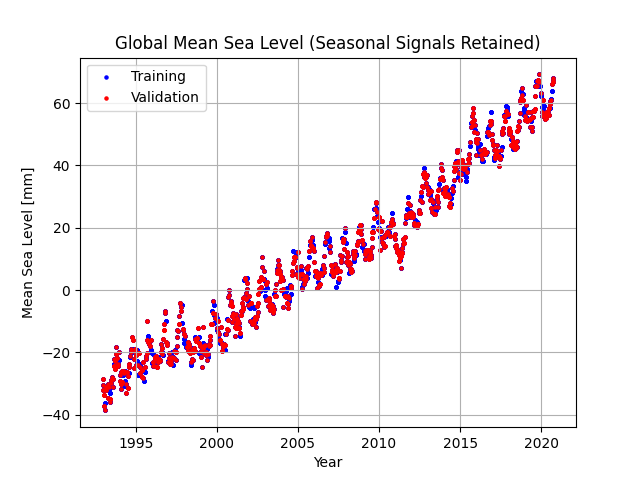
\includegraphics[width=\columnwidth]{figures/dataset.png}
	\label{fig:part_a}
\end{figure}

It can be seen there is a clear linear trend between year and mean sea level. The dataset was then partitioned into an 80/20 split of training and validation data. Applying linear regression to the (normalized) training data learned a line with an $b=0.9758$ and $w=0.9758$.

\LST{part\_a}

\begin{figure}[htpb]
	\centering
	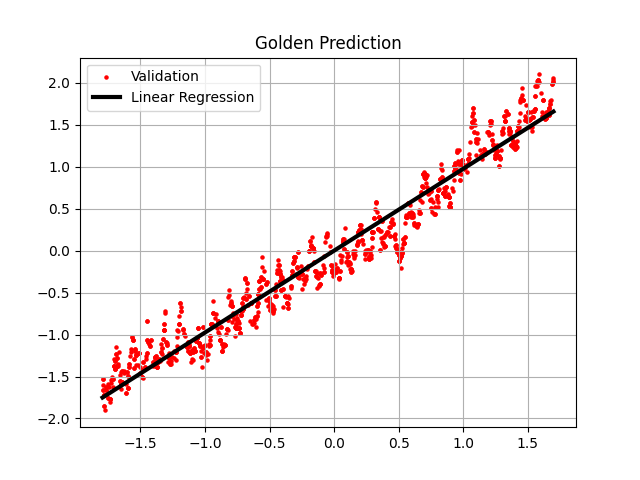
\includegraphics[width=\columnwidth]{figures/linear_regression.png}
	\label{fig:part_a}
\end{figure}

The regression line was found to have a MSE of $0.0489$